%%
%% Automatically generated file from DocOnce source
%% (https://github.com/hplgit/doconce/)
%%

% #define PREAMBLE

% #ifdef PREAMBLE
%-------------------- begin preamble ----------------------

\documentclass[%
oneside,                 % oneside: electronic viewing, twoside: printing
final,                   % draft: marks overfull hboxes, figures with paths
10pt]{article}

\listfiles               %  print all files needed to compile this document

\usepackage{relsize,makeidx,color,setspace,amsmath,amsfonts,amssymb}
\usepackage[table]{xcolor}
\usepackage{bm,ltablex,microtype}

\usepackage[pdftex]{graphicx}

% Packages for typesetting blocks of computer code
\usepackage{fancyvrb,framed,moreverb}

% Define colors
\definecolor{orange}{cmyk}{0,0.4,0.8,0.2}
\definecolor{tucorange}{rgb}{1.0,0.64,0}
\definecolor{darkorange}{rgb}{.71,0.21,0.01}
\definecolor{darkgreen}{rgb}{.12,.54,.11}
\definecolor{myteal}{rgb}{.26, .44, .56}
\definecolor{gray}{gray}{0.45}
\definecolor{mediumgray}{gray}{.8}
\definecolor{lightgray}{gray}{.95}
\definecolor{brown}{rgb}{0.54,0.27,0.07}
\definecolor{purple}{rgb}{0.5,0.0,0.5}
\definecolor{darkgray}{gray}{0.25}
\definecolor{darkblue}{rgb}{0,0.08,0.45}
\definecolor{darkblue2}{rgb}{0,0,0.8}
\definecolor{lightred}{rgb}{1.0,0.39,0.28}
\definecolor{lightgreen}{rgb}{0.48,0.99,0.0}
\definecolor{lightblue}{rgb}{0.53,0.81,0.92}
\definecolor{lightblue2}{rgb}{0.3,0.3,1.0}
\definecolor{lightpurple}{rgb}{0.87,0.63,0.87}
\definecolor{lightcyan}{rgb}{0.5,1.0,0.83}

\colorlet{comment_green}{green!50!black}
\colorlet{string_red}{red!60!black}
\colorlet{keyword_pink}{magenta!70!black}
\colorlet{indendifier_green}{green!70!white}

% Backgrounds for code
\definecolor{cbg_gray}{rgb}{.95, .95, .95}
\definecolor{bar_gray}{rgb}{.92, .92, .92}

\definecolor{cbg_yellowgray}{rgb}{.95, .95, .85}
\definecolor{bar_yellowgray}{rgb}{.95, .95, .65}

\colorlet{cbg_yellow2}{yellow!10}
\colorlet{bar_yellow2}{yellow!20}

\definecolor{cbg_yellow1}{rgb}{.98, .98, 0.8}
\definecolor{bar_yellow1}{rgb}{.98, .98, 0.4}

\definecolor{cbg_red1}{rgb}{1, 0.85, 0.85}
\definecolor{bar_red1}{rgb}{1, 0.75, 0.85}

\definecolor{cbg_blue1}{rgb}{0.87843, 0.95686, 1.0}
\definecolor{bar_blue1}{rgb}{0.7,     0.95686, 1}

\usepackage{listingsutf8}

% Common lstlisting parameters

\usepackage{calc}
\newlength{\lstboxwidth}  % width of lst box
\newlength{\framethickness}
\setlength{\framethickness}{0.5mm}
% for frame=trbl and a framerule that has significant size, set
% xleftmargin=5mm and xrightmargin=5mm.

\lstset{
  basicstyle=\small \ttfamily,
  breaklines=false,          % break/wrap lines
  breakatwhitespace=true,    % let linebreaks happen at whitespace
  breakindent=40pt,
  tab=,
  tabsize=4,                 % tab means 4 spaces
  %belowskip=\smallskipamount,  % space between code and text below
  xleftmargin=2mm,           % indentation of code frame
  xrightmargin=0mm,
  framexleftmargin=2mm,      % add frame space to the left of the code box
  %numbers=left,             % put line numbers on the left
  %stepnumber=2,             % stepnumber=1 numbers each line, =n every n lines
  framerule=\framethickness, % thickness of frame
  aboveskip=2ex,             % vertical space above code frame
  showstringspaces=false,    % show spaces in strings with an underscore
  showspaces=false,          % show spaces with an underscore
  showtabs=false,
  keepspaces=true,
  columns=fullflexible,      % tighter character kerning, like verb
  escapeinside={(*@}{@*)},   % (*@ \pause @*) in slides and math in code blocks
  extendedchars=\true,       % allows non-ascii chars, does not work with utf-8
}

% Internally defined styles for lstlisting

% Use this one without additional background color
\lstdefinestyle{blue1}{              % blue1 background for code snippets
backgroundcolor=\color{cbg_blue1},
}

% Use this one without additional background color
% (same as blue1, but with bar_blue1 frame)
\lstdefinestyle{blue1bar}{           % blue1 background for complete programs
backgroundcolor=\color{cbg_blue1},
frame=tb,                            % include frame
rulecolor=\color{bar_blue1},         % frame color
}

% Use this one without additional background color
\lstdefinestyle{gray}{
backgroundcolor=\color{cbg_gray},
%frame=tb,                            % include frame
%framerule=0.4pt                      % thickness of frame
rulecolor=\color{black!40},           % frame color
}

\lstdefinestyle{simple}{
commentstyle={},
}

% end of custom lstdefinestyles

\usepackage[T1]{fontenc}
%\usepackage[latin1]{inputenc}
\usepackage{ucs}
\usepackage[utf8x]{inputenc}

\usepackage{lmodern}         % Latin Modern fonts derived from Computer Modern

% Hyperlinks in PDF:
\definecolor{linkcolor}{rgb}{0,0,0.4}
\usepackage{hyperref}
\hypersetup{
    breaklinks=true,
    colorlinks=true,
    linkcolor=linkcolor,
    urlcolor=linkcolor,
    citecolor=black,
    filecolor=black,
    %filecolor=blue,
    pdfmenubar=true,
    pdftoolbar=true,
    bookmarksdepth=3   % Uncomment (and tweak) for PDF bookmarks with more levels than the TOC
    }
%\hyperbaseurl{}   % hyperlinks are relative to this root

\setcounter{tocdepth}{2}  % levels in table of contents

%\VerbatimFootnotes must come after hyperref and footmisc packages
\VerbatimFootnotes

% Tricks for having figures close to where they are defined:
% 1. define less restrictive rules for where to put figures
\setcounter{topnumber}{2}
\setcounter{bottomnumber}{2}
\setcounter{totalnumber}{4}
\renewcommand{\topfraction}{0.95}
\renewcommand{\bottomfraction}{0.95}
\renewcommand{\textfraction}{0}
\renewcommand{\floatpagefraction}{0.75}
% floatpagefraction must always be less than topfraction!
% 2. ensure all figures are flushed before next section
\usepackage[section]{placeins}
% 3. enable begin{figure}[H] (often leads to ugly pagebreaks)
%\usepackage{float}\restylefloat{figure}

% --- fancyhdr package for fancy headers ---
\usepackage{fancyhdr}
\fancyhf{} % sets both header and footer to nothing
\renewcommand{\headrulewidth}{0pt}
\fancyfoot[LE,RO]{\thepage}
% Ensure copyright on titlepage (article style) and chapter pages (book style)
\fancypagestyle{plain}{
  \fancyhf{}
  \fancyfoot[C]{{\footnotesize \copyright\ 2018-2019, Christian Forssén. Released under CC Attribution-NonCommercial 4.0 license}}
%  \renewcommand{\footrulewidth}{0mm}
  \renewcommand{\headrulewidth}{0mm}
}
% Ensure copyright on titlepages with \thispagestyle{empty}
\fancypagestyle{empty}{
  \fancyhf{}
  \fancyfoot[C]{{\footnotesize \copyright\ 2018-2019, Christian Forssén. Released under CC Attribution-NonCommercial 4.0 license}}
  \renewcommand{\footrulewidth}{0mm}
  \renewcommand{\headrulewidth}{0mm}
}

\pagestyle{fancy}


\usepackage[framemethod=TikZ]{mdframed}

% --- begin definitions of admonition environments ---

% Admonition style "mdfbox" is an oval colored box based on mdframed
% "notice" admon
\definecolor{mdfbox_notice_background}{rgb}{1,1,1}
\newmdenv[
  skipabove=15pt,
  skipbelow=15pt,
  outerlinewidth=0,
  backgroundcolor=mdfbox_notice_background,
  linecolor=black,
  linewidth=2pt,       % frame thickness
  frametitlebackgroundcolor=mdfbox_notice_background,
  frametitlerule=true,
  frametitlefont=\normalfont\bfseries,
  shadow=false,        % frame shadow?
  shadowsize=11pt,
  leftmargin=0,
  rightmargin=0,
  roundcorner=5,
  needspace=0pt,
]{notice_mdfboxmdframed}

\newenvironment{notice_mdfboxadmon}[1][]{
\begin{notice_mdfboxmdframed}[frametitle=#1]
}
{
\end{notice_mdfboxmdframed}
}

% Admonition style "mdfbox" is an oval colored box based on mdframed
% "summary" admon
\definecolor{mdfbox_summary_background}{rgb}{1,1,1}
\newmdenv[
  skipabove=15pt,
  skipbelow=15pt,
  outerlinewidth=0,
  backgroundcolor=mdfbox_summary_background,
  linecolor=black,
  linewidth=2pt,       % frame thickness
  frametitlebackgroundcolor=mdfbox_summary_background,
  frametitlerule=true,
  frametitlefont=\normalfont\bfseries,
  shadow=false,        % frame shadow?
  shadowsize=11pt,
  leftmargin=0,
  rightmargin=0,
  roundcorner=5,
  needspace=0pt,
]{summary_mdfboxmdframed}

\newenvironment{summary_mdfboxadmon}[1][]{
\begin{summary_mdfboxmdframed}[frametitle=#1]
}
{
\end{summary_mdfboxmdframed}
}

% Admonition style "mdfbox" is an oval colored box based on mdframed
% "warning" admon
\definecolor{mdfbox_warning_background}{rgb}{1,1,1}
\newmdenv[
  skipabove=15pt,
  skipbelow=15pt,
  outerlinewidth=0,
  backgroundcolor=mdfbox_warning_background,
  linecolor=black,
  linewidth=2pt,       % frame thickness
  frametitlebackgroundcolor=mdfbox_warning_background,
  frametitlerule=true,
  frametitlefont=\normalfont\bfseries,
  shadow=false,        % frame shadow?
  shadowsize=11pt,
  leftmargin=0,
  rightmargin=0,
  roundcorner=5,
  needspace=0pt,
]{warning_mdfboxmdframed}

\newenvironment{warning_mdfboxadmon}[1][]{
\begin{warning_mdfboxmdframed}[frametitle=#1]
}
{
\end{warning_mdfboxmdframed}
}

% Admonition style "mdfbox" is an oval colored box based on mdframed
% "question" admon
\definecolor{mdfbox_question_background}{rgb}{1,1,1}
\newmdenv[
  skipabove=15pt,
  skipbelow=15pt,
  outerlinewidth=0,
  backgroundcolor=mdfbox_question_background,
  linecolor=black,
  linewidth=2pt,       % frame thickness
  frametitlebackgroundcolor=mdfbox_question_background,
  frametitlerule=true,
  frametitlefont=\normalfont\bfseries,
  shadow=false,        % frame shadow?
  shadowsize=11pt,
  leftmargin=0,
  rightmargin=0,
  roundcorner=5,
  needspace=0pt,
]{question_mdfboxmdframed}

\newenvironment{question_mdfboxadmon}[1][]{
\begin{question_mdfboxmdframed}[frametitle=#1]
}
{
\end{question_mdfboxmdframed}
}

% Admonition style "mdfbox" is an oval colored box based on mdframed
% "block" admon
\definecolor{mdfbox_block_background}{rgb}{1,1,1}
\newmdenv[
  skipabove=15pt,
  skipbelow=15pt,
  outerlinewidth=0,
  backgroundcolor=mdfbox_block_background,
  linecolor=black,
  linewidth=2pt,       % frame thickness
  frametitlebackgroundcolor=mdfbox_block_background,
  frametitlerule=true,
  frametitlefont=\normalfont\bfseries,
  shadow=false,        % frame shadow?
  shadowsize=11pt,
  leftmargin=0,
  rightmargin=0,
  roundcorner=5,
  needspace=0pt,
]{block_mdfboxmdframed}

\newenvironment{block_mdfboxadmon}[1][]{
\begin{block_mdfboxmdframed}[frametitle=#1]
}
{
\end{block_mdfboxmdframed}
}

% --- end of definitions of admonition environments ---

% prevent orhpans and widows
\clubpenalty = 10000
\widowpenalty = 10000

% --- end of standard preamble for documents ---


\usepackage[swedish]{babel}

\raggedbottom
\makeindex
\usepackage[totoc]{idxlayout}   % for index in the toc
\usepackage[nottoc]{tocbibind}  % for references/bibliography in the toc

%-------------------- end preamble ----------------------

\begin{document}

% matching end for #ifdef PREAMBLE
% #endif

\newcommand{\exercisesection}[1]{\subsection*{#1}}

\input{newcommands_keep}

% ------------------- main content ----------------------



% ----------------- title -------------------------

\thispagestyle{empty}

\begin{center}
{\LARGE\bf
\begin{spacing}{1.25}
Learning from data: Bayesian Parameter Estimation
\end{spacing}
}
\end{center}

% ----------------- author(s) -------------------------

\begin{center}
{\bf Christian Forssén}
\end{center}

    \begin{center}
% List of all institutions:
\centerline{{\small Department of Physics, Chalmers University of Technology, Sweden}}
\end{center}
    
% ----------------- end author(s) -------------------------

% --- begin date ---
\begin{center}
Sep 16, 2019
\end{center}
% --- end date ---

\vspace{1cm}


% !split

\begin{figure}[!ht]  % fig:gw
  \centerline{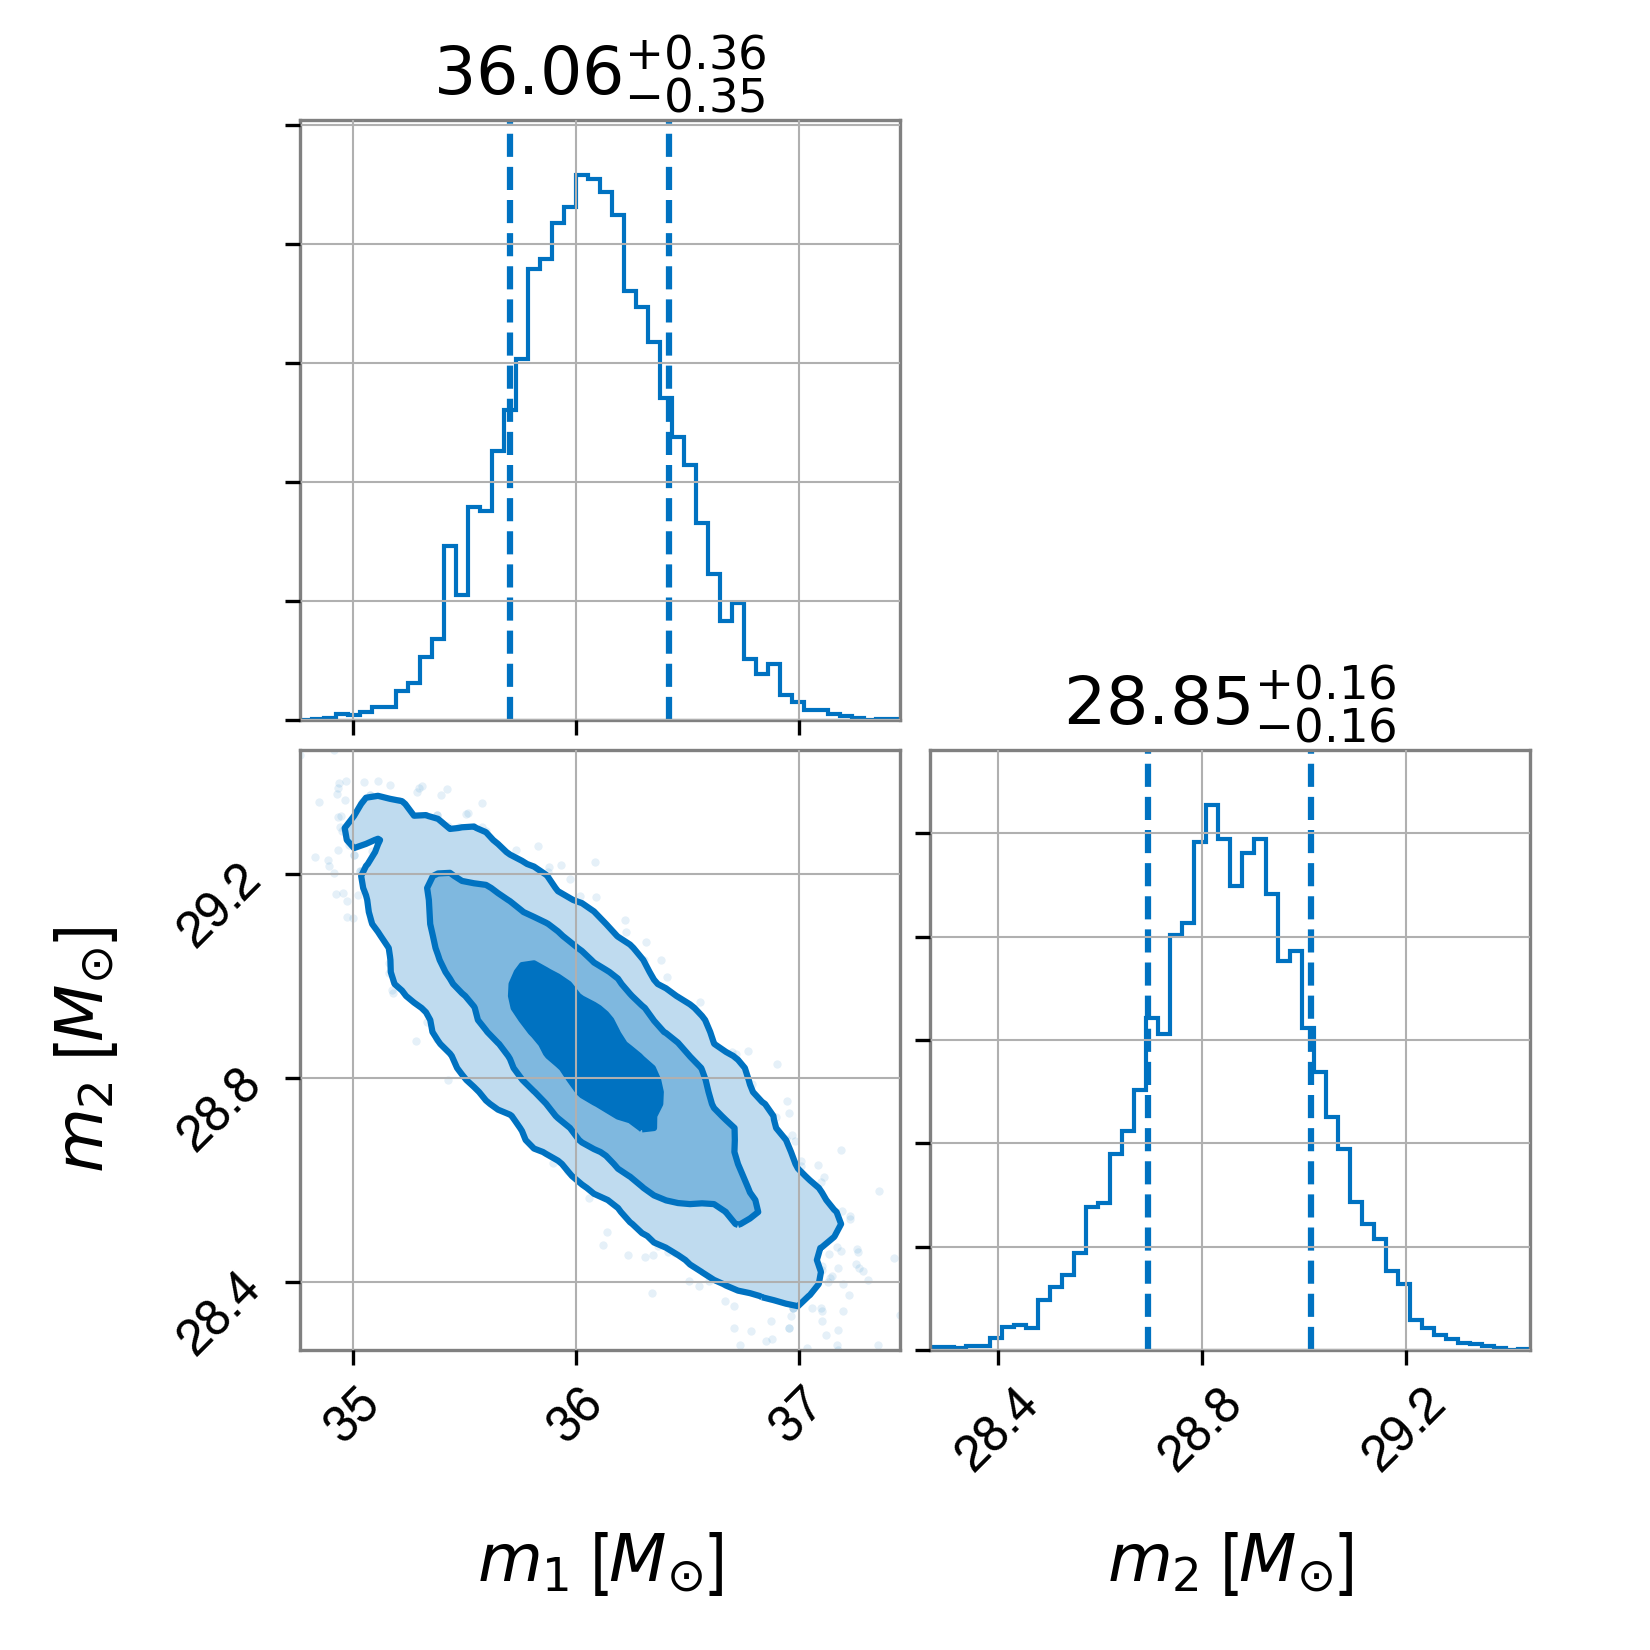
\includegraphics[width=0.8\linewidth]{fig/m1m2.png}}
  \caption{
  Joint pdf for the masses of two black holes merging obtained from the data analysis of a gravitational wave signal. This representation of a joint pdf is known as a corner plot. \label{fig:gw}
  }
\end{figure}
%\clearpage % flush figures fig:gw


% !split
\section{Inference With Parametric Models}

\begin{block_mdfboxadmon}[]
Inductive inference with parametric models is a very important tool in the natural sciences.
\begin{itemize}
\item Consider $N$ different models $M_i$ ($i = 1, \ldots, N$), each with parameters $\boldsymbol{\theta}_i$. Each of them implies a sampling distribution for possible data
\end{itemize}

\noindent
\[
p(D|\boldsymbol{\theta}_i, M_i)
\]

\begin{itemize}
\item The likelihood function is the pdf of the actual, observed data ($D_\mathrm{obs}$) given a set of parameters $\boldsymbol{\theta}_i$:
\end{itemize}

\noindent
\[
\mathcal{L}_i (\boldsymbol{\theta}_i) \equiv p(D_\mathrm{obs}|\boldsymbol{\theta}_i, M_i)
\]
\begin{itemize}
\item We may be uncertain about $M_i$ (model uncertainty),

\item or uncertain about $\boldsymbol{\theta}_i$ (parameter uncertainty).
\end{itemize}

\noindent
\end{block_mdfboxadmon} % title: 



% !split

\begin{block_mdfboxadmon}[]
\begin{description}
\item[Parameter Estimation:] 
  Premise = We have chosen a model (say $M_1$)\\
  $\Rightarrow$ What can we say about its parameters $\boldsymbol{\theta}_1$?

\item[Model comparison:] 
  Premise = We have a set of different models $\{M_i\}$\\
  $\Rightarrow$ How do they compare with each other? Do we have evidence to say that, e.g.~$M_1$, is better than the other models?

\item[Model adequacy:] 
  Premise = We have a model $M_1$\\
  $\Rightarrow$ Is $M_1$ adequate?

\item[Hybrid Uncertainty:] 
  Models share some common params: $\boldsymbol{\theta}_i = \{ \boldsymbol{\varphi}, \boldsymbol{\eta}_i\}$\\
  $\Rightarrow$ What can we say about $\boldsymbol{\varphi}$? (Systematic error is an example)
\end{description}

\noindent
\end{block_mdfboxadmon} % title: 



% !split
\subsection{Parameter estimation}

\begin{block_mdfboxadmon}[]
Overview comments:
\begin{itemize}
\item In general terms, ``parameter estimation'' in physics means obtaining values for parameters (constants) that appear in a theoretical model which describes data (exceptions to this general definition exist of course).

\item Conventionally this process is known as ``parameter fitting'' and the goal is to find the ``best fit''.

\item We will make particular interpretations of these phrases from our Bayesian point of view.

\item We will also see how familiar ideas like ``least-squares optimization'' show up from a Bayesian perspective.
\end{itemize}

\noindent
\end{block_mdfboxadmon} % title: 




% !split
\subsection{Bayesian parameter estimation}

\begin{block_mdfboxadmon}[]
We will now consider the very important task of model parameter estimation using statistical inference. 

Let us first remind ourselves what can go wrong in a fit. We have encountered both \textbf{underfitting} (model is not complex enough to describe the variability in the data) and \textbf{overfitting} (model tunes to data fluctuations, or terms are underdetermined causing them playing off each other). Bayesian methods can prevent/identify both these situations.
\end{block_mdfboxadmon} % title: 



% !split
% ===== Example: Measured flux from a star (single parameter) =====
\section{Example: Measured flux from a star (single parameter)}
Adapted from the blog \href{{http://jakevdp.github.io}}{Pythonic Perambulations} by Jake VanderPlas.

Imagine that we point our telescope to the sky, and observe the light coming from a single star. Our physics model will be that the star's true flux is constant with time, i.e.~that  it has a fixed value $F_\mathrm{true}$ (we'll also ignore effects like sky noise and other sources of systematic error). Thus, we have a single model parameter: $F_\mathrm{true}$.

We'll assume that we perform a series of $N$ measurements with our telescope, where the i:th measurement reports an observed photon flux $F_i$ and is accompanied by an error model given by $e_i$\footnote{We'll make the reasonable assumption that errors are Gaussian. In a Frequentist perspective, $e_i$ is the standard deviation of the results of a single measurement event in the limit of repetitions of \emph{that event}. In the Bayesian perspective, $e_i$ is the standard deviation of the (Gaussian) probability distribution describing our knowledge of that particular measurement given its observed value.}.
The question is, given this set of measurements $D = \{F_i\}_{i=0}^{N-1}$, and the statistical model $F_i = F_\mathrm{true} + e_i$, what is our best estimate of the true flux $F_\mathrm{true}$?



Because the measurements are number counts, a Poisson distribution is a good approximation to the measurement process:

\begin{lstlisting}[language=Python,style=blue1]
import numpy as np
from scipy import stats
import matplotlib.pyplot as plt
import emcee
\end{lstlisting}

\begin{lstlisting}[language=Python,style=blue1]
np.random.seed(1)      # for repeatability
F_true = 1000          # true flux, say number of photons measured in 1 second
N = 50                 # number of measurements
F = stats.poisson(F_true).rvs(N)
                       # N measurements of the flux
e = np.sqrt(F)         # errors on Poisson counts estimated via square root
\end{lstlisting}

Now let's make a simple visualization of the ``observed'' data, see Fig.~\ref{fig:flux}.

\begin{lstlisting}[language=Python,style=blue1]
fig, ax = plt.subplots()
ax.errorbar(F, np.arange(N), xerr=e, fmt='ok', ecolor='gray', alpha=0.5)
ax.vlines([F_true], 0, N, linewidth=5, alpha=0.2)
ax.set_xlabel("Flux");ax.set_ylabel("measurement number");
\end{lstlisting}


\begin{figure}[!ht]  % fig:flux
  \centerline{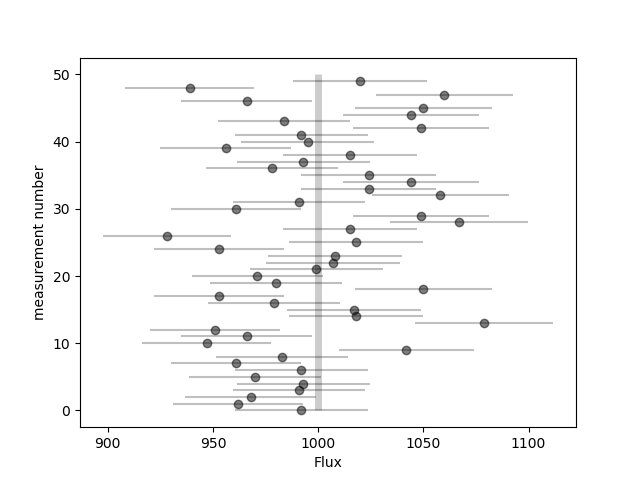
\includegraphics[width=0.8\linewidth]{fig/singlephotoncount_fig_1.png}}
  \caption{
  Single photon counts (flux measurements). \label{fig:flux}
  }
\end{figure}
%\clearpage % flush figures fig:flux


These measurements each have a different error $e_i$ which is estimated from Poisson statistics using the standard square-root rule. In this toy example we know the true flux that was used to generate the data, but the question is this: given our measurements and statistical model, what is our best estimate of $F_\mathrm{true}$?

Let's take a look at the frequentist and Bayesian approaches to solving this.

\paragraph{Simple Photon Counts: Frequentist Approach.}
We'll start with the classical frequentist maximum likelihood approach. Given a single observation $D_i = F_i$, we can compute the probability distribution of the measurement given the true flux $F_\mathrm{true}$ given our assumption of Gaussian errors
\begin{equation}
p(D_i | F_\mathrm{true}, I) = \frac{1}{\sqrt{2\pi e_i^2}} \exp \left( \frac{-(F_i-F_\mathrm{true})^2}{2e_i^2} \right).
\end{equation}
This should be read ``the probability of $D_i$ given $F_\mathrm{true}$
equals ...''. You should recognize this as a normal distribution with mean $F_\mathrm{true}$ and standard deviation $e_i$.

We construct the \emph{likelihood function} by computing the product of the probabilities for each data point
\begin{equation}
\mathcal{L}(F_\mathrm{true}) = \prod_{i=1}^N p(D_i | F_\mathrm{true}, I),
\end{equation}
here $D = \{D_i\}$ represents the entire set of measurements. Because the value of the likelihood can become very small, it is often more convenient to instead compute the log-likelihood. 


\begin{notice_mdfboxadmon}[Notice]
In the following we will use $\log$ to denote the natural logarithm. We will write $\log_{10}$ if we specifically mean the logarithm with base 10.
\end{notice_mdfboxadmon} % title: Notice



Combining the previous two equations and computing the log, we have
\begin{equation}
\log\mathcal{L} = -\frac{1}{2} \sum_{i=1}^N \left[ \log(2\pi e_i^2) +  \frac{(F_i-F_\mathrm{true})^2}{e_i^2} \right].
\end{equation}

What we'd like to do is determine $F_\mathrm{true}$ such that the likelihood is maximized. At this pont we can note that that problem of maximizing the likelihood is equivalent to the minimization of the sum
\begin{equation}
\sum_{i=1}^N \frac{(F_i-F_\mathrm{true})^2}{e_i^2},
\end{equation}
which you should recognize as the chi-squared function encountered in the linear regression model.

Therefore, it is not surprising that this particular maximization problem can be solved analytically (i.e.~by setting $d\log\mathcal{L}/d F_\mathrm{true} = 0$). This results in the following observed estimate of $F_\mathrm{true}$
\begin{equation}
F_\mathrm{est} = \frac{ \sum_{i=1}^N w_i F_i }{ \sum_{i=1}^N w_i}, \quad w_i = 1/e_i^2.
\end{equation}
Notice that in the special case of all errors $e_i$ being equal, this reduces to
\begin{equation}
F_\mathrm{est} = \frac{1}{N} \sum_{i=1} F_i.
\end{equation}
That is, in agreement with intuition, $F_\mathrm{est}$ is simply the mean of the observed data when errors are equal.

We can go further and ask what the error of our estimate is. In the frequentist approach, this can be accomplished by fitting a Gaussian approximation to the likelihood curve at maximum; in this simple case this can also be solved analytically (the sum of Gaussians is also a Gaussian). It can be shown that the standard deviation of this Gaussian approximation is $\sigma_\mathrm{est}$, which is given by
\begin{equation}
\frac{ 1 } {\sigma_\mathrm{est}^2} = \sum_{i=1}^N w_i .
\end{equation}
These results are fairly simple calculations; let's evaluate them for our toy dataset:

\begin{lstlisting}[language=Python,style=blue1]
w=1./e**2
print(f"""
F_true = {F_true}
F_est = {(w * F).sum() / w.sum():.0f} +/- { w.sum() ** -0.5:.0f} (based on {N} measurements) """)
\end{lstlisting}
\Verb!F_true = 1000! \\
\Verb!F_est = 998 +/- 4 (based on 50 measurements)! \\

We find that for 50 measurements of the flux, our estimate has an error of about 0.4\% and is consistent with the input value.


\paragraph{Simple Photon Counts: Bayesian Approach.}
The Bayesian approach, as you might expect, begins and ends with probabilities. Our hypothesis is that the star has a constant flux $F_\mathrm{true}$. It recognizes that what we fundamentally want to compute is our knowledge of the parameter in question given the data and other information (such as our knowledge of uncertainties for the observed values), i.e.~in this case, $p(F_\mathrm{true} | D,I)$.
Note that this formulation of the problem is fundamentally contrary to the frequentist philosophy, which says that probabilities have no meaning for model parameters like $F_\mathrm{true}$. Nevertheless, within the Bayesian philosophy this is perfectly acceptable.

To compute this pdf, Bayesians next apply Bayes' Theorem.
If we set the prior $p(F_\mathrm{true}|I) \propto 1$ (a flat prior), we find
$p(F_\mathrm{true}|D,I) \propto p(D | F_\mathrm{true},I) \equiv \mathcal{L}(F_\mathrm{true})$
and the Bayesian probability is maximized at precisely the same value as the frequentist result! So despite the philosophical differences, we see that (for this simple problem at least) the Bayesian and frequentist point estimates are equivalent.

\paragraph{A note about priors.}
The prior allows inclusion of other information into the computation, which becomes very useful in cases where multiple measurement strategies are being combined to constrain a single model. The necessity to specify a prior, however, is one of the more controversial pieces of Bayesian analysis.
A frequentist will point out that the prior is problematic when no true prior information is available. Though it might seem straightforward to use a noninformative prior like the flat prior mentioned above, there are some \href{{http://normaldeviate.wordpress.com/2013/07/13/lost-causes-in-statistics-ii-noninformative- priors/comment-page-1/}}{surprisingly subtleties} involved. It turns out that in many situations, a truly noninformative prior does not exist! Frequentists point out that the subjective choice of a prior which necessarily biases your result has no place in statistical data analysis.
A Bayesian would counter that frequentism doesn't solve this problem, but simply skirts the question. Frequentism can often be viewed as simply a special case of the Bayesian approach for some (implicit) choice of the prior: a Bayesian would say that it's better to make this implicit choice explicit, even if the choice might include some subjectivity.

\paragraph{Simple Photon Counts: Bayesian approach in practice.}
Leaving these philosophical debates aside for the time being, let's address how Bayesian results are generally computed in practice. For a one parameter problem like the one considered here, it's as simple as computing the posterior probability $p(F_\mathrm{true} | D,I)$ as a function of $F_\mathrm{true}$: this is the distribution reflecting our knowledge of the parameter $F_\mathrm{true}$.
But as the dimension of the model grows, this direct approach becomes increasingly intractable. For this reason, Bayesian calculations often depend on sampling methods such as Markov Chain Monte Carlo (MCMC). For this practical example, let us apply an MCMC approach using Dan Foreman-Mackey's \href{{http://dan.iel.fm/emcee/current/}}{emcee} package. Keep in mind here that the goal is to generate a set of points drawn from the posterior probability distribution, and to use those points to determine the answer we seek.
To perform this MCMC, we start by defining Python functions for the prior $p(F_\mathrm{true} | I)$, the likelihood $p(D | F_\mathrm{true},I)$, and the posterior $p(F_\mathrm{true} | D,I)$, noting that none of these need be properly normalized. Our model here is one-dimensional, but to handle multi-dimensional models we'll define the model in terms of an array of parameters $\boldsymbol{\theta}$, which in this case is $\boldsymbol{\theta} = [F_\mathrm{true}]$

\begin{lstlisting}[language=Python,style=blue1]
def log_prior(theta):
    if theta>0 and theta<10000:
        return 0 # flat prior
    else:
        return -np.inf

def log_likelihood(theta, F, e):
    return -0.5 * np.sum(np.log(2 * np.pi * e ** 2) \ 
                             + (F - theta[0]) ** 2 / e ** 2)
                             
def log_posterior(theta, F, e):
    return log_prior(theta) + log_likelihood(theta, F, e)
\end{lstlisting}

Now we set up the problem, including generating some random starting guesses for the multiple chains of points.

\begin{lstlisting}[language=Python,style=blue1]
ndim = 1      # number of parameters in the model
nwalkers = 50 # number of MCMC walkers
nwarm = 1000  # "warm-up" period to let chains stabilize
nsteps = 2000 # number of MCMC steps to take
# we'll start at random locations between 0 and 2000
starting_guesses = 2000 * np.random.rand(nwalkers, ndim)
sampler = emcee.EnsembleSampler(nwalkers, ndim, log_posterior, args=[F,e])
sampler.run_mcmc(starting_guesses, nsteps)
# Shape of sampler.chain  = (nwalkers, nsteps, ndim)
# Flatten the sampler chain and discard warm-in points:
samples = sampler.chain[:, nwarm:, :].reshape((-1, ndim))
\end{lstlisting}

If this all worked correctly, the array sample should contain a series of 50,000 points drawn from the posterior. Let's plot them and check. See results in Fig.~\ref{fig:flux-bayesian}.

\begin{lstlisting}[language=Python,style=blue1]
fig, ax = plt.subplots()
ax.hist(samples, bins=50, histtype="stepfilled", alpha=0.3, density=True)
ax.set_xlabel(r'$F_\mathrm{est}$')
ax.set_ylabel(r'$p(F_\mathrm{est}|D,I)$');
\end{lstlisting}

\begin{figure}[!ht]  % fig:flux-bayesian
  \centerline{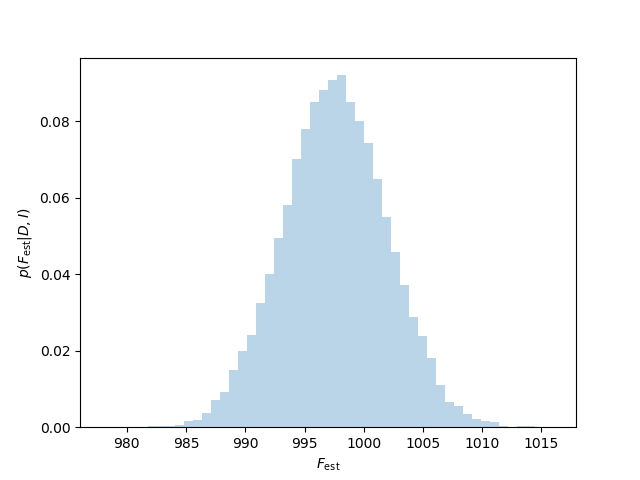
\includegraphics[width=0.8\linewidth]{fig/singlephotoncount_fig_2.png}}
  \caption{
  Bayesian posterior pdf (represented by a histogram of MCMC samples) from flux measurements. \label{fig:flux-bayesian}
  }
\end{figure}
%\clearpage % flush figures fig:flux-bayesian


% !split
\subsection{Aside: Best estimates and confidence intervals}
The posterior distribution from our Bayesian data analysis is the key quantity that encodes our inference about the values of the model parameters, given the data and the relevant background information. Often, however, we wish to summarize this result with just a few numbers: the best estimate and a measure of its reliability. 

There are a few different options for this. The choice of the most appropriate one depends mainly on the shape of the posterior distribution:

% !split
\paragraph{Symmetric posterior pdfs.}
Since the probability (density) associated with any particular value of the parameter is a measure of how much we believe that it lies in the neighbourhood of that point, our best estimate is given by the maximum of the posterior pdf. If we denote the quantity of interest by $\theta$, with a posterior pdf $P =p(\theta|D,I)$, then the best estimate of its value $\theta_0$ is given by the condition $dP/d\theta|_{\theta=\theta_0}=0$. Strictly speaking, we should also check the sign of the second derivative to ensure that $\theta_0$ represents a maximum.

To obtain a measure of the reliability of this best estimate, we need to look at the width or spread of the posterior pdf about $\theta_0$. When considering the behaviour of any function in the neighbourhood of a particular point, it is often helpful to carry out a Taylor series expansion; this is simply a standard tool for (locally) approximating a complicated function by a low-order polynomial. The linear term is zero at the maximum and the quadratic term is often the dominating one determining the width of the posterior pdf. Ignoring all the higher-order terms we arrive at the Gaussian approximation (see more details below)
\begin{equation}
p(\theta|D,I) \approx \frac{1}{\sigma\sqrt{2\pi}} \exp \left[ -\frac{(\theta-\mu)^2}{2\sigma^2} \right],
\end{equation}
where the mean $\mu = \theta_0$ and the variance $\sigma = \left( - \left. \frac{d^2L}{d\theta^2} \right|_{\theta_0} \right)^{-1/2}$, where $L$ is the logarithm of the posterior $P$. Our inference about the quantity of interest is conveyed very concisely, therefore, by the 67\% Bayesian confidence interval $\theta = \theta_0 \pm \sigma$, and 
\[
p(\theta_0-\sigma < \theta < \theta_0+\sigma | D,I) = \int_{\theta_0-\sigma}^{\theta_0+\sigma} p(\theta|D,I) d\theta \approx 0.67.
\]

% !split
\paragraph{Asymmetric posterior pdfs.}
While the maximum of the posterior ($\theta_0$) can still be regarded as giving the best estimate, the true value is now more likely to be on one side of this rather than the other. Alternatively one can compute the mean value, $\langle \theta \rangle = \int \theta p(\theta|D,I) d\theta$, although this tends to overemphasise very long tails. The best option is probably a compromise that can be employed when having access to a large sample from the posterior (as provided by an MCMC), namely to give the median of this ensemble.

Furthermore, the concept of an error-bar does not seem appropriate in this case, as it implicitly entails the idea of symmetry. A good way of expressing the reliability with which a parameter can be inferred, for an asymmetric posterior pdf, is rather through a \emph{confidence interval}. Since the area under the posterior pdf between $\theta_1$ and $\theta_2$ is proportional to how much we believe that $\theta$ lies in that range, the shortest interval that encloses 67\% of the area represents a sensible measure of the uncertainty of the estimate. Obviously we can choose to provide some other degree-of-belief that we think is relevant for the case at hand. Assuming that the posterior pdf has been normalized, to have unit area, we need to find $\theta_1$ and $\theta_2$ such that: 
\[
p(\theta_1 < \theta < \theta_2 | D,I) = \int_{\theta_1}^{\theta_2} p(\theta|D,I) d\theta \approx 0.67, 
\]
where the difference $\theta_2 - \theta_1$ is as small as possible. The region $\theta_1 < \theta < \theta_2$ is then called the shortest 67\% confidence interval. 

% !split
\paragraph{Multimodal posterior pdfs.}
We can sometimes obtain posteriors which are multimodal; i.e.~contains several disconnected regions with large probabilities. There is no difficulty when one of the maxima is very much larger than the others: we can simply ignore the subsidiary solutions, to a good approximation, and concentrate on the global maximum. The problem arises when there are several maxima of comparable magnitude. What do we now mean by a best estimate, and how should we quantify its reliability? The idea of a best estimate and an error-bar, or even a confidence interval, is merely an attempt to summarize the posterior with just two or three numbers; sometimes this just can’t be done, and so these concepts are not valid. For the bimodal case we might be able to characterize the posterior in terms of a few numbers: two best estimates and their associated error-bars, or disjoint confidence intervals. For a general multimodal pdf, the most honest thing we can do is just display the posterior itself.


\begin{block_mdfboxadmon}[]
Two options for assigning credible intervals to asymmetric and multimodal pdfs:
\begin{itemize}
\item Equal-tailed interval: the probability area above and below the interval are equal.

\item Highest posterior density (HPD) interval: The posterior density for any point within the interval is larger than the posterior density for any point outside the interval.
\end{itemize}

\noindent
\end{block_mdfboxadmon} % title: 




% !split
\paragraph{Different views on confidence intervals.}

\begin{block_mdfboxadmon}[]
A Bayesian confidence interval, or credible interval, or degree-of-belief (DOB) interval is the following: Given this data and other information there is $d \%$ probability that this interval contains the true value of the parameter. E.g.~a 95\% DOB interval implies that the Baysian data analyser would bet 20-to-1 that the true result is inside the interval.
\end{block_mdfboxadmon} % title: 



% !split

\begin{block_mdfboxadmon}[]
A frequentist 95\% confidence interval should be understood as follows: 
``There is a 95\% probability that when I compute a confidence interval from data of this sort that he true value of the parameter will fall within the (hypothetical) space of observations''. So the parameter is fixed (no pdf) and the confidence interval is based on random sampling of data. 

Let's try again to understand this: If we make a large number of repeated samples, then 95\% of the intervals extracted in this way will include the true value of the parameter.
\end{block_mdfboxadmon} % title: 




\paragraph{Simple Photon Counts: Best estimates and confidence intervals.}
To compute these numbers for our example, you would run:

\begin{lstlisting}[language=Python,style=blue1]
sampper=np.percentile(samples, [2.5, 16.5, 50, 83.5, 97.5],axis=0).flatten()
print(f"""
F_true = {F_true}
Based on {N} measurements the posterior point estimates are:
...F_est = { np.mean(samples):.0f} +/- { np.std(samples):.0f}
or using credibility intervals:
...F_est = {sampper[2]:.0f}          (posterior median) 
...F_est in [{sampper[1]:.0f}, {sampper[3]:.0f}] (67% credibility interval) 
...F_est in [{sampper[0]:.0f}, {sampper[4]:.0f}] (95% credibility interval) """)
\end{lstlisting}
\Verb!F_true = 1000! \\
\texttt{Based on 50 measurements the posterior point estimates are:} \\
\Verb!...F_est = 998 +/- 4! \\
\texttt{or using credibility intervals:} \\
\Verb!...F_est = 998          (posterior median)!  \\
\Verb!...F_est in [993, 1002] (67% credibility interval)!  \\
\Verb!...F_est in [989, 1006] (95% credibility interval)!  \\

In this particular example, the posterior pdf is actually a Gaussian (since it is constructed as a product of Gaussians), and the mean and variance from the quadratic approximation will agree exactly with the frequentist approach.

From this final result you might come away with the impression that the Bayesian method is unnecessarily complicated, and in this case it certainly is. Using an MCMC sampler to characterize a one-dimensional normal distribution is a bit like using the Death Star to destroy a beach ball, but we did this here because it demonstrates an approach that can scale to complicated posteriors in many, many dimensions, and can provide nice results in more complicated situations where an analytic likelihood approach is not possible.

Furthermore, as data and models grow in complexity, the two approaches can diverge greatly. 



% !split
\section{Example: Gaussian noise and averages}
The example in the demonstration notebook is from Sivia's book. How do we infer the mean and standard deviation of a Gaussian distribution from $M$ measurements $D \in \{ x_k \}_{k=0}^{M-1}$ that should be distributed according to a normal distribution $p( D | \mu,\sigma,I)$?

% !split
Start from Bayes theorem
\[
p(\mu,\sigma | D, I) = \frac{p(D|\mu,\sigma,I) p(\mu,\sigma|I)}{p(D|I)}
\]
\begin{itemize}
\item Remind yourself about the names of the different terms.

\item It should become intuitive what the different probabilities (pdfs) describe.

\item Bayes theorem tells you how to flip from (hard-to-compute) $p(\mu,\sigma | D, I) \Leftrightarrow p(D|\mu,\sigma,I)$ (easier-to-compute).
\end{itemize}

\noindent
% !split
Aside on the denominator, which is known as the ``data probability'' or ``marginalized likelihood'' or ``evidence''. 
\begin{itemize}
\item With $\theta$ denoting a general vector of parameters we must have
\end{itemize}

\noindent
\[
p(D|I) = \int d\theta p(D|\theta,I) p(\theta|I).
\]
\begin{itemize}
\item This integration (or marginalization) over all parameters is often difficult to perform.

\item Fortunately, for \textbf{parameter estimation} we don't need $p(D|I)$ since it doesn't depend on $\theta$. We usually only need relative probabilities, or we can determine the normalization $N$ after we have computed the unnormalized posterior 
\end{itemize}

\noindent
\[
p(\theta | D,I) = \frac{1}{N} p(D|\theta,I) p(\theta|I).
\]

% !split
If we use a uniform prior $p(\theta | I ) \propto 1$ (in a finite volume), then the posterior is proportional to the \textbf{likelihood}
\[
p(\theta | D,I) \propto p(D|\theta,I) = \mathcal{L}(\theta)
\]
In this particular situation, the mode of the likelihood (which would correspond to the point estimate of maximum likelihood) is equivalent to the mode of the posterior pdf in the Bayesian analysis.

% !split
The real use of the prior, however, is to include into the analysis any additional information that you might have. The prior statement makes such additional assumptions and information very explicit.

But how do we actually compute the posterior in practice. Most often we won't be able to get an analytical expression, but we can sample the distribution using a method known as Markov Chain Monte Carlo (MCMC).

% !split
\section{Example: Fitting a straight line}
The next example that we will study is the well known fit of a straight line.

\begin{itemize}
\item Here the theoretical model is
\end{itemize}

\noindent
\[
y_\mathrm{th}(x; \theta) = m x + b,
\]
with parameters $\theta = [b,m]$.

\begin{itemize}
\item The statistical model for the data is
\end{itemize}

\noindent
\[
y_{\mathrm{exp},i} = y_{\mathrm{th},i} + \delta y_{\mathrm{exp},i},
\]
where we often assume that the experimental errors are independent and normally distributed so that
\[
y_i = \mathcal{N} \left( y_\mathrm{th}(x_i; \theta), e_i^2 \right).
\]

\begin{itemize}
\item Is independent errors always a good approximation?

\item An even better statistical model for theoretical models with a quantified, finite resolution would be
\end{itemize}

\noindent
\[
y_\mathrm{exp} = y_\mathrm{th} + \delta y_\mathrm{exp} + \delta y_\mathrm{th}.
\]

% !split
\paragraph{Why normal distributions?}
Let us give a quick motivation why Gaussian distributions show up so often. Say that we have a pdf $p(\theta | D,I)$. Our best estimate from this pdf will be $\theta_0$ where
\[ 
\left. 
\frac{ \partial p }{ \partial \theta }
\right|_{\theta_0} = 0, \qquad
\left. \frac{ \partial^2 p }{ \partial \theta^2 }
\right|_{\theta_0} < 0.
\]
The distribution usually varies very rapidly so we study $L(\theta) \equiv \log p$ instead.
Near the peak, it behaves as
\[
L(\theta) = L(\theta_0) + \frac{1}{2} \left. \frac{\partial^2 L}{\partial \theta^2} \right|_{\theta_0} \left( \theta - \theta_0 \right)^2 + \ldots,
\]
where the first-order term is zero since we are expanding around a maximum and $\partial L / \partial\theta = 0$.

% !split
If we neglect higher-order terms we find that 
\[
p(\theta|D,I) \approx A \exp \left[ \frac{1}{2} \left. \frac{\partial^2 L}{\partial \theta^2} \right|_{\theta_0} \left( \theta - \theta_0 \right)^2  \right],
\]
which is a Gaussian $\mathcal{N}(\mu,\sigma^2)$ with
\[
\mu = \theta_0, \qquad \sigma^2 = \left( - \left. \frac{\partial^2 L}{\partial \theta^2} \right|_{\theta_0} \right)^{-1/2}.
\]

% !split
\subsection{Correlations}
In the ``fitting a straight-line'' example you should find that the joint pdf for the slope and the intercept $[m, b]$ corresponds to a slanted ellipse. That result implies that the model parameters are \textbf{correlated}.

\begin{itemize}
\item Try to understand the correlation that you find in this example.
\end{itemize}

\noindent
Let us explore correlations by studying the behavior of the pdf at the maximum.
A Taylor expansion for a bivariate pdf $p(x,y)$ around the mode $(x_0,y_0)$ gives
\[
p(x,y) \approx p(x_0,y_0) + \frac{1}{2} \begin{pmatrix} x-x_0 & y-y_0 \end{pmatrix}
H
\begin{pmatrix} x-x_0 \\ y-y_0 \end{pmatrix},
\]
where $H$ is the symmetric Hessian matrix
\[
\begin{pmatrix}
A & C \\ C & B
\end{pmatrix}, 
\]
with elements
\[
A = \left. \frac{\partial^2 p}{\partial x^2} \right|_{x_0,y_0}, \quad
B = \left. \frac{\partial^2 p}{\partial y^2} \right|_{x_0,y_0}, \quad
C = \left. \frac{\partial^2 p}{\partial x \partial y} \right|_{x_0,y_0}.
\]


% !split
\begin{itemize}
\item So in this quadratic approximation the contour is an ellipse centered at $(x_0,y_0)$ with orientation and eccentricity determined by $A,B,C$.

\item The principal axes are found from the eigenvectors of $H$.

\item Depending on the skewness of the ellipse, the parameters are either (i) not correlated, (ii) correlated, or (iii) anti-correlated.

\item Take a minute to consider what that implies.
\end{itemize}

\noindent

% ------------------- end of main content ---------------

% #ifdef PREAMBLE
\end{document}
% #endif

